\documentclass[border=0.8ex,svgnames,tikz]{standalone}
\usepackage{amsmath,mathtools}
\usepackage{fontspec}
\setmainfont{Source Serif 4}
\setsansfont{Source Sans 3}
\setmonofont{Source Code Pro}
\usetikzlibrary{calc,positioning}
\begin{document}
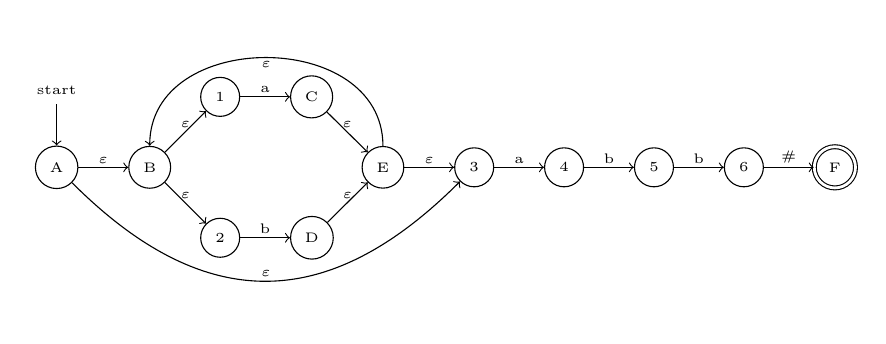
\begin{tikzpicture}
  % NFA
  \node[](start){\tiny start};
  \node[circle, draw=black, below=1.5em of start](A){\tiny A};
  \node[circle, draw=black, right=1.8em of A](B){\tiny B};
  \node[circle, draw=black, above right=2.1em of B](1){\tiny 1};
  \node[circle, draw=black, below right=2.1em of B](2){\tiny 2};
  \node[circle, draw=black, right=1.8em of 1](C){\tiny C};
  \node[circle, draw=black, right=1.8em of 2](D){\tiny D};
  \node[circle, draw=black, right=1.8em of $(C)!0.5!(D)$](E){\tiny E};
  \node[circle, draw=black, right=1.8em of E](3){\tiny 3};
  \node[circle, draw=black, right=1.8em of 3](4){\tiny 4};
  \node[circle, draw=black, right=1.8em of 4](5){\tiny 5};
  \node[circle, draw=black, right=1.8em of 5](6){\tiny 6};
  \node[circle, double, double distance=1pt, draw=black, right=1.8em of 6](F){\tiny F};

  \path[->]
  (start) edge (A)
  (A) edge[out=315, in=225, min distance=6.75em] node[above=-2pt]{\tiny $\varepsilon$} (3)
  (A) edge node[above=-2pt]{\tiny $\varepsilon$} (B)
  (B) edge node[above=-2pt]{\tiny $\varepsilon$} (1)
  (1) edge node[above=-2pt]{\tiny a} (C)
  (C) edge node[above=-2pt]{\tiny $\varepsilon$} (E)
  (B) edge node[above=-2pt]{\tiny $\varepsilon$} (2)
  (2) edge node[above=-2pt]{\tiny b} (D)
  (D) edge node[above=-2pt]{\tiny $\varepsilon$} (E)
  (E) edge[out=90, in=90, min distance=4.25em] node[below=-2pt]{\tiny $\varepsilon$} (B)
  (E) edge node[above=-2pt]{\tiny $\varepsilon$} (3)
  (3) edge node[above=-2pt]{\tiny a} (4)
  (4) edge node[above=-2pt]{\tiny b} (5)
  (5) edge node[above=-2pt]{\tiny b} (6)
  (6) edge node[above=-2pt]{\tiny \#} (F);
\end{tikzpicture}
\end{document}
